\chapter{Introduction}
\label{cha:introduction}

The world's population is growing each year. 
Making healthcare more efficient and robust is of great importance in order to handle the challenges that arises with a growing population.
One way of increasing the efficiency as well as the quality of healthcare is to create automated systems that can aid doctors in their process.
As the population is growing it is of utmost importance to ensure that the quality of diagnoses remain high, and to minimize the risk of missing some critical piece of information.
Taking advantage of the available medical information is key to create aforementioned systems.

Information pertaining to a patient's diagnosis is often in the form of written clinical reports.
This is one example of information that can be utilized in automated systems, by extracting information from old reports, the process of writing new ones can be enriched.
A system could show cases with similar features as the one currently being written, the doctor could then compare the findings and check if they have obtained an abnormal result.
Being able to perform such a comparison will result in extra quality assurance in the diagnostic flow.
It could also provide doctors with more confidence in that their diagnosis is correct.

The problem systems like this would face is to categorize medical reports in order to make further suggestions.
One approach that is commonly used for such problems is machine learning.
Machine learning is a field where a set of inputs is used to create a mapping to some output values~\cite{bishop2006pattern}.
This is done by using data to build a, usually statistical, model.

The task of predicting a category, or class, for a given text document is called text classification.
Text classification is usually solved using supervised learning~\cite{aggarwal2012surveyclass}. 
In supervised text classification, there exists a set of inputs, in this case text data, that already has a category assigned to it.
This data is then used to fit the model so that it later make predictions for inputs that it has not yet been exposed to.
One model that have been shown to be successful in text classification is Support Vector Machines (SVM)~\cite{joachims1998text, aggarwal2012surveyclass, tong2001support}.

In order to fit a machine learning model to predict categories for clinical reports, we need a set of already categorized, or labeled, data.
That is, we need to assign categories to an existing set of clinical reports.
It is often the case that text data is widely available, but it is harder to come by data that is already labeled.
Obtaining high quality data is important to use in machine learning systems, both in healthcare and other areas.
Since the models require a sufficient amount of labeled reports, the task of labeling them can be cumbersome.
Especially in the case of clinical data, since doctors and other clinicians time is both valuable and expensive.
By improving the process and the quality of data to be labeled, and thereby reducing the number of reports that need to be categorized, they can spend more time doing their job.

A field within machine learning that is focused on the task of improving the data labeling process is called active learning.
It is a form of semi-supervised learning.
The algorithm queries an oracle (in this case a doctor) for labels for the data points that it think will help the model improve the most.
This is used when there is plenty of readily available data, but assigning labels is expensive.
Since the data points to be labeled are actively selected, the models can require fewer examples than if they were selected at random.
The points can be selected by considering the certainty of the models, and request to label the documents that the model is less certain about.
Another approach, which has not been given as much attention, is using the underlying structure of the data to select points.
The goal with this approach is to capture the distribution of the categories.

If one of two classes is assigned to each document, you have a binary classification problem~\cite{bishop2006pattern}.
Problems where one of several classes is assigned to an instance is called a multi-class classification problem.
Multi-labeled classification is when you assign one or more label to each document.
This thesis is mainly concerned with multi-label classification.
Assigning several classes to a document is more time consuming than in the cases where you only need to find one option.
In those cases the process can be stopped when the appropriate label has been found.
However, when a document can be assigned several classes the entirety of the text needs to be considered.
For example, a news article be on several subjects, such as both economics and sport.
Just because the category sport has been identified, the entire document has to be read in order to find any additional categories.
This makes the use of active learning to enhance the labeling of documents even more useful in the multi-labeled case.  

\section{Motivation}
\label{sec:motivation}

This thesis is carried out at Sectra Medical Imaging IT Solutions AB, as a part of their research group.
They are currently pursuing a research project with Region Skåne, which is responsible for the healthcare in Skåne, that is located in southern Sweden.
The intention behind the project is to use machine learning techniques to, among other things, be able to suggest categories to doctors while they are writing medical reports.
Another case is to use the categories of documents to present doctors with medical reports that are handling similar cases from the past.
With this information the doctors could get an extra quality assurance check in their diagnostic flow.

In order to build these system, you need a substantial amount of labeled clinical reports.
Therefore, the purpose of this thesis is to increase the quality and efficiency of the process of labeling these reports.
This will be done by using unsupervised learning techniques such as topic models and clustering to first remove documents that are not supposed to be labeled.
These invalid reports are documents that describe patients never showing up for a scan, deceased patients and patients being moved to a different hospital, among others.
For the labeling, a system is to be built to use active learning in conjunction with the aforementioned unsupervised techniques to increase the quality of the labeled documents.
In the work that they have done so far in the research project, the doctor that primarily worked with the labeling of reports stated that the distribution over the labeled categories is very skewed.
The vast majority of labeled documents were assigned the same few categories.
This in turn leads the models to require a lot of labeled samples to work well.
By using active learning we can reduce the number of labeled samples needed to obtain an accurate model.

\section{Aim}
\label{sec:aim}

The purpose with this thesis project is to evaluate different solutions to increase the quality of labeled reports, and thereby reducing the amount of them needed for use within the project.
Resulting from this will be a complete, standalone, system for labeling reports.
The reports are interactively queried so a user can label the reports that are deemed most useful by the system.
This will then be used together with an existing web interface that Sectra created for the purpose of labeling reports, which can be seen in Figure~\ref{fig:web-interface}.

\begin{figure}
      \centering
      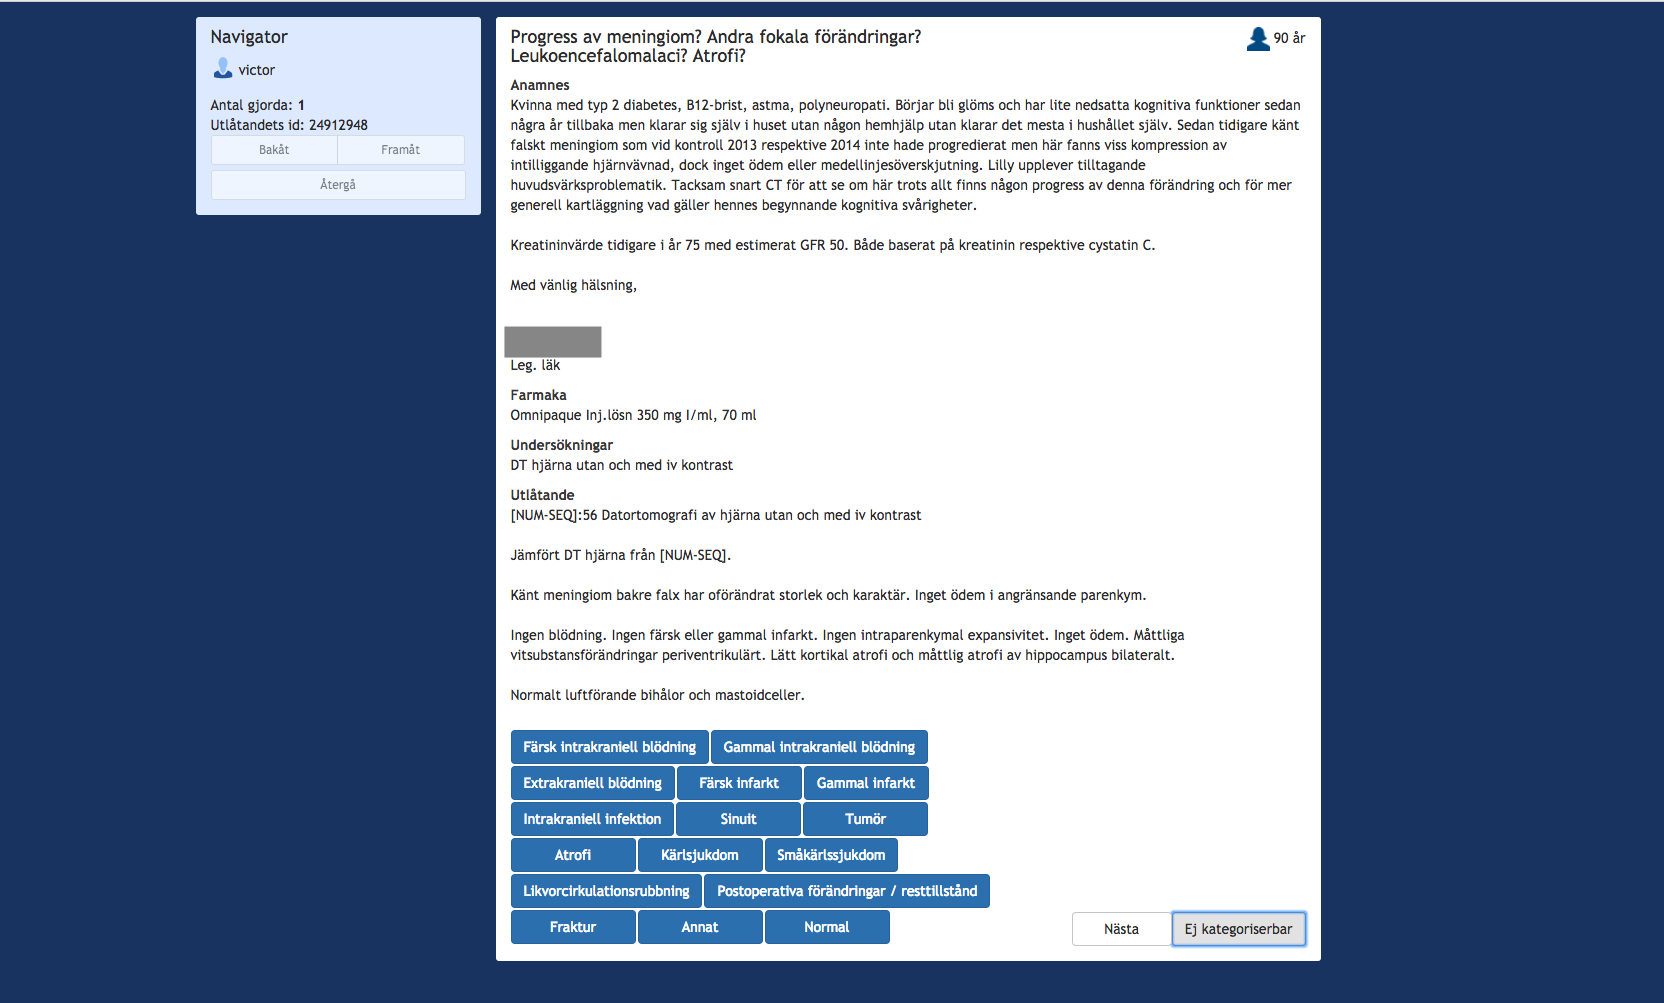
\includegraphics[scale=0.25]{web-interface}
      \caption{A screenshot of the interface used to label clinical reports at Sectra}
      \label{web-interface}
\end{figure}

\section{Research questions}
\label{sec:research-questions}

The specific research questions that this thesis will treat are presented here.
They will be the main focus of study.

\begin{enumerate}

\item \textit{Is it possible filter out invalid clinical reports by using an unsupervised techniques such as topic modeling?}
      \newline
      In the dataset from Sectra, there are reports describing patients not showing up for or changing the time of their appointments, deceased patients or patients that have been ordered to another hospital.
      These reports does not contain any information of value from a medical point of view and should not be considered in the report labeling process.

      Unsupervised machine learning models such as topic modeling does by definition not require any labeled documents to train on.
      If it is possible to, without any such data, to capture the necessary variance and group these invalid reports together and they can be removed from the labeling process before a doctor is presented with them that would be an additional hurdle removed from the process.

\item \label{intro:re-q2} 
      \textit{What active learning strategies are good alternatives to sample documents at random in a multi-label document labeling system? How well does these alternatives perform?}
      \newline
      How we are choosing the documents to be sampled is important.
      If the dataset that is being sampled is skewed, i.e. some categories are a more frequent than others, our labeled set will likely follow that distribution.
      This will result in models requiring a lot of labeled documents to gather a sufficient amount of reports that are of the less common categories.
      Without these, the model with only perform well on the frequently occurring categories.

      If the decision boundaries of our models can be used to pick documents that would be more informative for the model, the number of labeled documents could be reduced and still obtain the same performance.
      Another approach to selecting the documents to sample is to take advantage of the underlying structure of the data.

      The algorithms to be evaluated will be based on the models certainty, as well as taking advantage of the underlying structure of the data.
      When choosing the algorithm to use, there are several different factors that will affect the final results, and therefore need to be taken into consideration.
      How well the models perform on the data will be evaluated based on the accuracy, precision, recall and f1-score of the models.
      But they also need to be able to query documents in a reasonable time, if it is expensive to label reports it is likely to be expensive to wait for the reports to be queried.
      If the algorithm needs a big initial set of labeled reports is another factor that will be evaluated.

  \item \label{intro:re-q3}
      \textit{How does the algorithms from question~\ref{intro:re-q2} effect the balance of labels in the labeled dataset?}
      Another indication on the quality of the labeled reports is the balance between the classes.
      Based on the initial sampling, the underlying distribution of labels in the clinical data is far from uniform.
      There are certain categories, like the one describing that everything is okay with the patient, that is a lot more common than other more rare illnesses.
      Even though the original data may be imbalanced, selecting samples that contains a better balance between the different categories could improve the performance of the models.

      The goal here is to see which one of the different sampling techniques that will result in the best balance between the different categories in the resulting dataset.
      The best balance being the one with the smallest ratio between the most common, and the least common labels.
\end{enumerate}

\section{Delimitations}
\label{sec:delimitations}

Even though the sampling strategies are evaluated objectively on the Reuters dataset, the applicability of the techniques on clinical data is only evaluated by one physician, on the one dataset provided by Sectra.

\section{Structure of the Report}
\label{sec:structure}

The next chapter covers the background theory that is relevant for the thesis.
After the theory, the methodology used is described, which is followed by a chapter covering the results.
The method and results are then discussed in Chapter~\ref{cha:discussion}.
Finally, Chapter~\ref{cha:conclusion} presents the conclusions.
